\documentclass[12pt,a4paper]{article}

% ----------------- Paquetes -----------------
\usepackage[utf8]{inputenc}
\usepackage[spanish]{babel}
\usepackage[a4paper,top=2.5cm,bottom=2.5cm,left=3cm,right=3cm]{geometry}
\usepackage{setspace}
\usepackage{graphicx}
\usepackage{amsmath}
\usepackage{titlesec}
\usepackage{url}
\usepackage{enumitem}
\usepackage{multicol}
\usepackage{helvet} % Arial-like font
\usepackage{comment}
% ----------------- Fuente Arial -----------------
% Load the biblatex package
\usepackage[backend=biber, style=numeric]{biblatex}
% Add your .bib file
\usepackage{fancyhdr} % Encabezado y pie de página
\renewcommand{\familydefault}{\sfdefault}
% ----------------- Fuente Arial -----------------

% ----------------- Interlineado 1.5 -----------------
\onehalfspacing

% ----------------- Estilos de sección -----------------
\titleformat{\section}{\bfseries\fontsize{14}{16}\selectfont}{\thesection}{1em}{}
\titleformat{\subsection}{\bfseries\fontsize{12}{14}\selectfont}{\thesubsection}{1em}{}

% ----------------- Pie de página -----------------
\pagestyle{fancy}
\fancyhf{} % Limpia encabezados y pies
\fancyfoot[L]{\fontsize{10}{12}\selectfont Electrónica de Potencia, IE-AD26}
\fancyfoot[R]{\fontsize{10}{12}\selectfont Dr. Luis Alejandro Flores Oropeza}
\renewcommand{\headrulewidth}{0pt} % sin línea en encabezado
\renewcommand{\footrulewidth}{0pt} % sin línea en pie de página

%-- Das comm --
\newcommand{\titulos}[3]{
  {\fontsize{12}{14}\bfseries \textit{#1}}\\
  {\fontsize{10}{12}\normalfont #2}\\
  {\fontsize{9}{11}\itshape #3}\\[0.5cm]

}


\usepackage{subcaption}

\begin{document}

\begin{center}
  {\fontsize{16}{18}\bfseries Convertidor Boost 24V-127V}\\[0.5cm]
  %english
  {\fontsize{14}{16}\itshape Boost converter 24V-127V}\\[1cm] 
  \begin{multicols}{2}
    \titulos{Contreras Reyes Orlando}{Universidad Autónoma de Aguascalientes}{al348390@edu.uaa.mx}

    \titulos{García Barrera Iker Emiliano}{Universidad Autónoma de Aguascalientes}{al307630@edu.uaa.mx}

    \titulos{Lara Hernández Kevin Adrián}{Universidad Autónoma de Aguascalientes}{al46437@edu.uaa.mx}

    \titulos{Jiménez de Luna Rafael Odín}{Universidad Autónoma de Aguascalientes}{al332461@edu.uaa.mx}

  \end{multicols}
\end{center}
\section*{Resumen}
Se diseñó, simuló y construyó un convertidor boost para elevar un voltaje de $24\,\mathrm{V}$ a $127\,\mathrm{V}$ con una potencia de $100\,\mathrm{W}$. Se seleccionaron los componentes adecuados, se validó el diseño mediante simulación en LTSpice y se realizaron pruebas experimentales para confirmar el correcto funcionamiento del convertidor. Se discutieron las dificultades encontradas durante el proceso y se proporcionaron sugerencias para futuras implementaciones.

\noindent \textbf{Palabras clave:} Capacitor, convertidor boost, LTSpice, simulación, diseño de circuitos, validación experimental.

\section*{Abstract}
\emph{Designed, simulated, and built a boost converter to step up a voltage from $24\,\mathrm{V}$ to $127\,\mathrm{V}$ with a power of $100\,\mathrm{W}$. Selected appropriate components, validated the design through LTSpice simulation, and conducted experimental tests to confirm the correct operation of the converter. Discussed difficulties encountered during the process and provided suggestions for future implementations.}

\noindent \textbf{Keywords:} Boost converter, Capacitor, LTSpice, simulation, circuit design, experimental validation.
\newpage
\section{Materiales}

\begin{itemize}
    \item IC TL494
    \item IC IR2110 Driver 
    \item MOSFET IRF740
    \item Resistores:
    \begin{itemize}
    \item 2 unidades de $10\,\mathrm{k\Omega}$
    \item 1 unidad de $1\,\mathrm{k\Omega}$
    \item 1 unidad de $2\,\mathrm{k\Omega}$
\end{itemize}
\item Capacitores:
    \begin{itemize}
    \item 1 unidad de $1\,\mathrm{nF}$
    \item 1 unidad de $470\,\mathrm{nF}$
    \item 1 unidades de $100\,\mathrm{nF}$
    \item 1 unidades de $1\,\mathrm{uF}$
    \item 1 unidades de $33\,\mathrm{uF}$

\end{itemize}
    \item Diodo MUR460
    \item Inductor $220\,\mu\mathrm{H}$
\end{itemize}




\section{Metodología}
 
\subsection{Cálculo de los componentes}
Considerando un voltaje de entrada de $24\,\mathrm{V}$ y un voltaje de salida de $127\,\mathrm{V}$ para alimentar un foco de $100\,\mathrm{W}$. Con una frecuencia definida de $100\,\mathrm{kHz}$, con un rizado de $10\%$ en el voltaje de salida y $25\%$ en la corriente del inductor, tomamos:
\[
V_i = 24\,\mathrm{V},\qquad V_o = 127\,\mathrm{V},\qquad f_s = 100\,\mathrm{kHz},\qquad \Delta i_L = 0.25\,I_o,\qquad \Delta v_o = 0.10\,V_o
\]
$$
\begin{align*}
d &= 1 - \dfrac{v_i}{v_o} = 1 - \dfrac{24}{127} = \dfrac{103}{127} \approx 0.8110\\[4pt]
I_L &= \dfrac{I_o}{1-d} = \dfrac{0.8}{1-0.8110} \approx 4.2333\ \mathrm{A}\\[4pt]
\Delta I &= 0.25\,I_L = 0.25\cdot 4.2333 \approx 1.0583\ \mathrm{A}\\[4pt]
C &= \dfrac{I_o\, d}{DV\, f} = \dfrac{0.8\cdot 0.8110}{1.27\cdot 100000} = 5.1088\times 10^{-6}\,\mathrm{F} \approx 5.11\,\mu\mathrm{F}; C = \boxed{5\,\mu\mathrm{F}} \\[4pt]
L &= \dfrac{v_i\, d}{f\, \Delta I} = \dfrac{24\cdot 0.8110}{100000\cdot 1.0583} = 1.8392\times 10^{-4}\,\mathrm{H} \approx 183.92\,\mu\mathrm{H} \approx \boxed{220\,\mu\mathrm{H}} 
\end{align*}
$$
Pese a que el capacitor calculado es de aproximadamente $5\,\mu\mathrm{F}$, se optó por utilizar un capacitor de $33\,\mu\mathrm{F}$ debido a que se considero un capacitor muy bajo para una aplicación real.

\section{Resultados}
Se armó el circuito que se muestra en la figura \ref{fig:esq}, se decidió implementar la parte de potencia (100 V) en una tarjeta perforada debido a que los cables deberían de ser lo suficientemente gruesos para soporta la corriente tal y como se ve en la figura \ref{fig:cir}.  
\begin{figure}[!h]
     \centering
     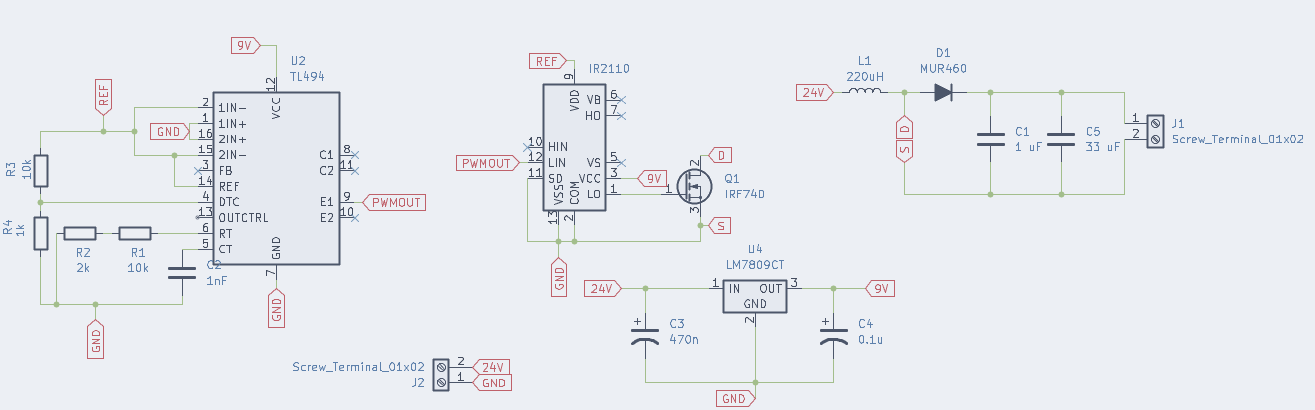
\includegraphics[width=1\linewidth]{AC/Esquemático.png}
     \caption{Esquemático del circuito implementado.}
     \label{fig:esq}
 \end{figure}

 \begin{figure}[!h]
     \centering
     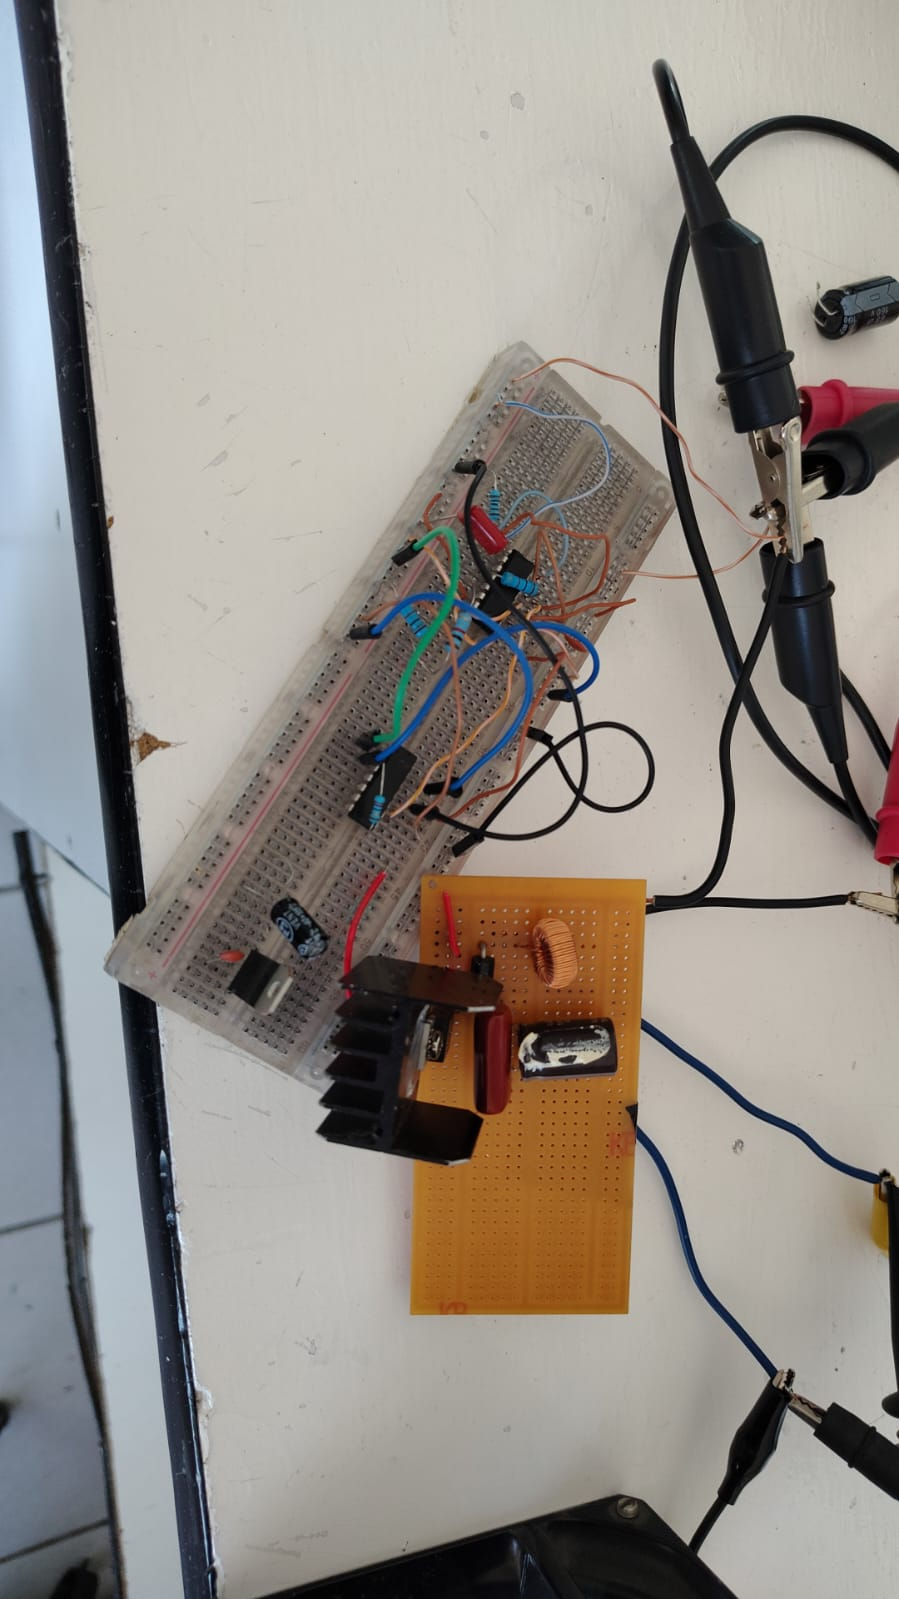
\includegraphics[width=0.5\linewidth,angle =90]{AC/EX2Circuit.png}
     \caption{Circuito implmentado}
     \label{fig:cir}
 \end{figure}
\subsection{Validación mediante Simulación}
 
Antes de la construcción física, se realizó una simulación completa del circuito utilizando el software LTSpice. Esto permitió verificar el comportamiento esperado del convertidor boost, identificar posibles errores de diseño y ajustar los valores de los componentes para optimizar el rendimiento antes de la implementación física.

A continuación, se presenta la simulación realizada en LTSpice en la Figura~\ref{fig:sim}. En la Figura~\ref{fig:onda} se muestra un zoom de la salida obtenida en la simulación, donde se puede observar claramente el umbral de voltaje de operación oscila entre $123\,\mathrm{V}$ y $128\,\mathrm{V}$, lo cual confirma que el diseño del convertidor boost es correcto y cumple con las especificaciones establecidas.
 
\begin{figure}[!h]
     \centering
    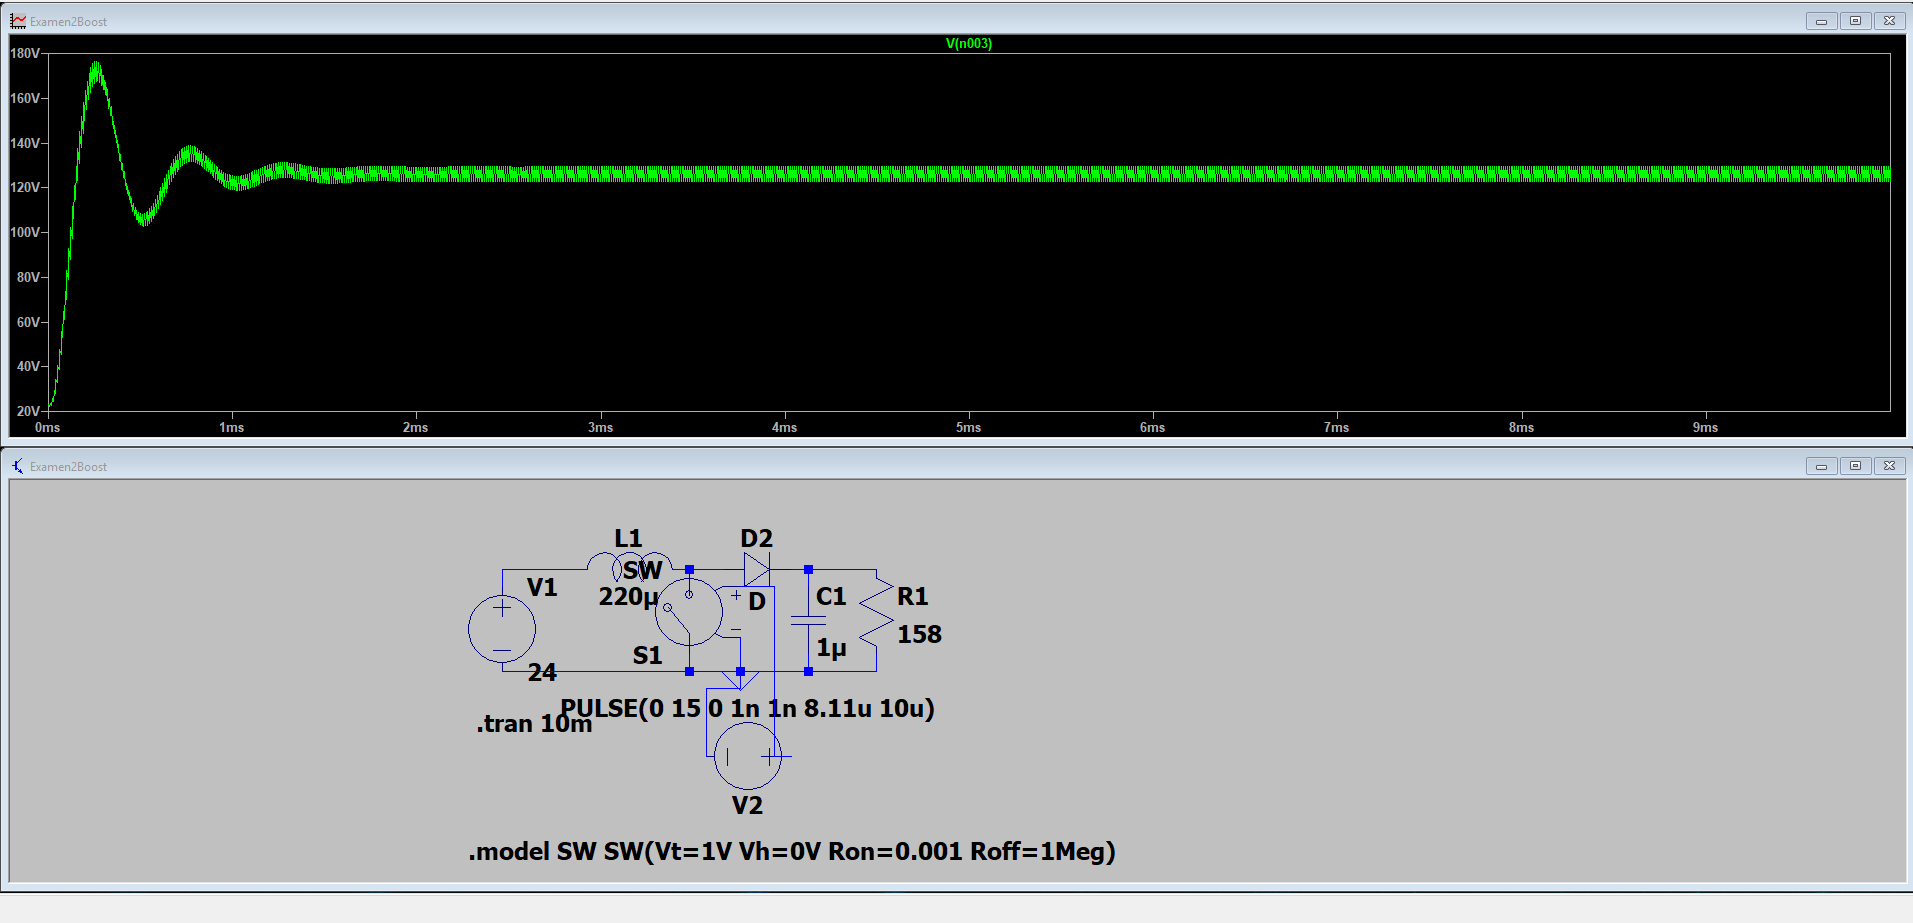
\includegraphics[width=0.75\linewidth]{AC/Spice2Ex.png}
    \caption{Esquemático con simulación en LTSpice.}
     \label{fig:sim}
 \end{figure}


 \begin{figure}[!h]
     \centering
    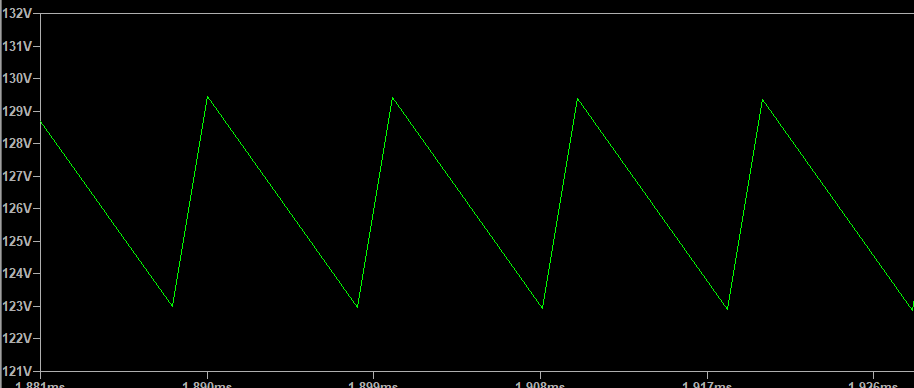
\includegraphics[width=0.9\linewidth]{AC/EX2Zoom.png}
     \caption{Zoom de la simulación.}
     \label{fig:onda}
 \end{figure}


 \newpage 
 
\subsection{Validación Experimental}
 
Una vez completada la construcción del prototipo, se procedió a validar experimentalmente el funcionamiento mediante mediciones con osciloscopio, comparando los resultados con las predicciones teóricas y simuladas, tal como se muestra en la Figura~\ref{fig:out}.
 
 
\begin{figure}[!h]
     \centering
      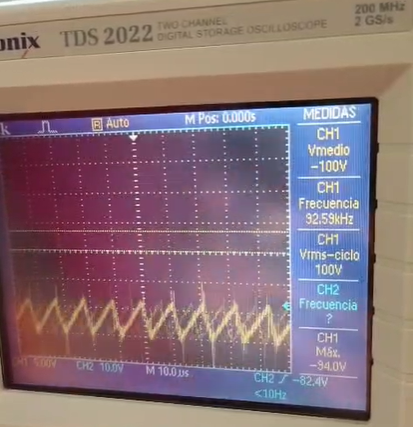
\includegraphics[width=0.75\linewidth]{AC/EX2Salida.png}
    \caption{Voltaje obtenido en pruebas experimentales.}
     \label{fig:out}
 \end{figure} 


\section{Discusión}
Durante el avance del proyecto tuvimos experiencias tanto positivas como complicadas. Una de las principales dificultades fue durante la etapa de simulación, ya que conectamos algunos elementos de forma incorrecta y eso ocasionó pérdida de tiempo mientras tratábamos de identificar el problema. Además, inicialmente utilizamos los valores calculados de manera ideal para el convertidor boost, pero descubrimos que estaban muy alejados de los valores que realmente funcionaban en la práctica.

Consideramos que una experiencia de aprendizaje aún más valiosa sería que desde un inicio se explicara a los estudiantes la diferencia entre los valores ideales y los valores reales, así como las razones detrás de estas diferencias. En nuestro caso, aprendimos esto mediante prueba y error. Por ejemplo, obtuvimos valores teóricos como un capacitor de 1 µF y un inductor de 220 mH, y al ver que el circuito no funcionaba pensamos que el problema estaba en los componentes o en las conexiones. Sin embargo, después comprendimos que esos valores ideales no necesariamente son funcionales en aplicaciones reales debido a pérdidas, limitaciones de componentes y otras condiciones prácticas.

Creemos que el trabajo realizado, junto con el reporte y toda la documentación generada, puede servir para que futuras generaciones desarrollen este proyecto de una forma más sencilla y eficiente. Nuestro objetivo es que puedan partir de una mejor referencia y lograr resultados aún mejores, por ejemplo, alcanzar el objetivo de elevar de 12 V a 120 V. En nuestro caso logramos elevar de 24 V a 110 V, por lo que consideramos que todavía hay espacio para mejorar y refinar el diseño.

A pesar de las dificultades, estamos agradecidos por la experiencia porque aprendimos mucho durante el proceso. El hecho de revisar circuitos, realizar pruebas y recalcular varias veces los valores nos ayudó a comprender mejor el funcionamiento del sistema. Aunque en algunos momentos no fue una experiencia sencilla, debido al tiempo extra invertido y las dificultades encontradas, consideramos que el aprendizaje obtenido fue significativo.

Como sugerencia para futuras generaciones, podría ser útil proporcionar algunas referencias iniciales, como valores aproximados que ya hayan funcionado, componentes recomendados, MOSFET, drivers o configuraciones previamente comprobadas. Esto serviría como guía y evitaría que los estudiantes tengan que comenzar toda la investigación desde cero, permitiendo enfocarse más en comprender y mejorar el proyecto.
\newpage
\section{Contreras Reyes Orlando}
Para mi algo  que aprendi fue sobre los distintos capacitores y su aplicación por lo que me gustaría anexar mi investigación sobre ello.
\subsection*{Selección de capacitores (cerámicos, electrolíticos y de poliéster)}
En un convertidor conmutado (como el boost), la elección del capacitor no depende solo de la capacitancia nominal; también influyen fuertemente parámetros como la resistencia serie equivalente (ESR), la inductancia serie equivalente (ESL), la corriente de rizado admisible, la estabilidad con temperatura/voltaje y la vida útil. En la práctica, suele combinarse más de un tipo de capacitor para cubrir diferentes rangos de frecuencia.

\paragraph{Capacitores cerámicos (MLCC).}
Son ideales para desacoplo de alta frecuencia por su muy baja ESL/ESR y buena respuesta en transitorios rápidos. Como limitación, en dieléctricos comunes de alta constante (p.\,ej. X5R/X7R) la capacitancia efectiva puede disminuir con el sesgo DC (DC bias) y con la temperatura; además, pueden presentar microfonía (efecto piezoeléctrico) y su valor útil depende del voltaje de operación.

\paragraph{Capacitores electrolíticos (aluminio).}
Son una opción típica para \textit{bulk} (almacenamiento de energía) por su alta capacitancia por costo. Sus limitaciones principales son ESR/ESL mayores (peor desempeño a altas frecuencias), envejecimiento por secado del electrolito (vida útil finita) y calentamiento por corriente de rizado; por ello, suelen complementarse con capacitores cerámicos cercanos a los nodos de conmutación.

\paragraph{Capacitores de poliéster (película, PET).}
Los capacitores de película (film) de poliéster se usan comúnmente cuando se requiere un comportamiento estable y buena capacidad de manejar pulsos. En general, presentan buena estabilidad del valor con el voltaje aplicado (sin caída por DC bias como en algunos cerámicos), son no polarizados y tienden a tener pérdidas relativamente bajas y buena tolerancia a $dv/dt$ para su tamaño. Como limitación, su capacitancia por volumen es menor que la de los electrolíticos, por lo que para valores grandes pueden volverse voluminosos.

\paragraph{Justificación del uso de dos capacitores de poliéster en el prototipo.}
En nuestro montaje se recurrió a capacitores de poliéster (dos piezas) principalmente porque ayudan a:
\begin{itemize}[nosep]
    \item reducir el rizado (por menor ESR) en comparación con un capacitor \textit{bulk} electrolítico típico de tamaño similar,
    \item mejorar la respuesta ante cambios de carga/perturbaciones (mejor soporte en transitorios),
    \item mantener un comportamiento más consistente del filtrado dentro del rango de operación, especialmente cuando se requiere un capacitor compacto.
\end{itemize}

\begin{table}[!h]
\centering
\renewcommand{\arraystretch}{1.25}
\begin{tabular}{p{3.2cm} p{5.7cm} p{5.7cm}}
\hline
\textbf{Tipo} & \textbf{Beneficios} & \textbf{Limitaciones / precauciones} \\
\hline
Cerámico (MLCC) &
Muy baja ESL/ESR; excelente para alta frecuencia y transitorios; ideal para desacoplo cercano a CI y nodos rápidos. &
Capacitancia efectiva puede caer con DC bias/temperatura (según dieléctrico); microfonía; valores grandes a alto voltaje pueden ser voluminosos/costosos. \\
\hline
Electrolítico (Al) &
Alta capacitancia por costo; buen \textit{bulk} para energía a baja frecuencia; común en entradas/salidas de fuentes. &
ESR/ESL mayores (peor en alta frecuencia); vida útil limitada por temperatura y rizado; tamaño mayor para buen desempeño. \\
\hline
Poliéster (film, PET) &
Estable con el voltaje; no polarizado; buena capacidad de manejar pulsos y transitorios; útil como capacitor de filtro intermedio y/o para reducir rizado junto con otros tipos. &
Menor capacitancia por volumen que un electrolítico; puede ser más grande para valores altos; típicamente no reemplaza al \textit{bulk} cuando se requiere mucha energía. \\
\hline
\end{tabular}
\caption{Comparativa cualitativa de capacitores usados comúnmente en filtrado y desacoplo.}
\label{tab:comparativa_capacitores}
\end{table}

\begin{figure}[!h]
    \centering
    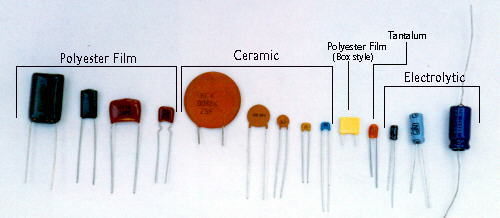
\includegraphics[width=0.8\linewidth]{AC/TiposCap.png}
    \caption{Tipos de Capacitores}
    \label{fig:placeholder}
\end{figure}
\newpage
\begin{thebibliography}{99}

\bibitem{ref1}
Capacitores. (2018, August 2). Ingenieros Por La Fisica. \url{https://programmingbeta.wordpress.com/capacitores/}

\bibitem{ref2}
Boylestad, R. L., \& Nashelsky, L. (2003). \textit{Dispositivos pnpn y otros}. En Electrónica: teoría de circuitos y dispositivos electrónicos (pp. 923-964). Pearson, Prentice Hall.

\bibitem{ref3}
Hayt, W. H., Kemmerly, J. E., \& Durbin, S. M. (2012). \textit{Capacitores e inductores}. En Análisis de circuitos en ingeniería (pp. 217-260). Mc Graw Hill.

\bibitem{ref4}
Tipos de capacitores. (2026). Industrias GSL. \url{https://industriasgsl.com/blogs/automatizacion/tipos-de-capacitores?srsltid=AfmBOoqDvtp-faEdklrTUsJ54tu3hh6dFANtO8Hsms3K1KiiqveIWiLV}

\bibitem{ref7}
Pini, A. (2020, September 17). Fundamentos: Comprender las características de los tipos de condensadores para utilizarlos de manera apropiada y segura. DigiKey; Editores de DigiKey de América del Norte. \url{https://www.digikey.com.mx/es/articles/fundamentals-understand-the-characteristics-of-capacitor-types?srsltid=AfmBOorVOmZmD0A5OOr2U9KFeEBZaVDdOKtmZ3YF0qdJqKAtNAGQlczK}s

\end{thebibliography}

\end{document}